
%(BEGIN_QUESTION)
% Copyright 2011, Tony R. Kuphaldt, released under the Creative Commons Attribution License (v 1.0)
% This means you may do almost anything with this work of mine, so long as you give me proper credit

Suppose a Rosemount model 3244MV (FOUNDATION Fieldbus) temperature transmitter is used as an electric current sensor, the transmitter configured for millivolt input and connected in parallel with a shunt resistor carrying load current in a DC power system.  The shunt resistor has a resistance of 35 milliohms:

$$\includegraphics[width=15.5cm]{i03642x01.eps}$$

Determine the proper {\tt XD\_Scale}, {\tt OUT\_Scale}, and {\tt L\_Type} parameter values to make the transmitter functional over a DC load current range of 0 to 2.5 amps.

\underbar{file i03642}
%(END_QUESTION)





%(BEGIN_ANSWER)

{\tt L\_Type} = Indirect

\vskip 10pt

{\tt XD\_Scale} = 0 to 87.5 mV

\vskip 10pt

{\tt OUT\_Scale} = 0 to 2.5 amps

%(END_ANSWER)





%(BEGIN_NOTES)


%INDEX% Fieldbus, instrument ranging: setting XD_Scale and OUT_Scale parameters for an application

%(END_NOTES)


